%-------------------------
% Resume in Latex
% Author : Arkadeep Das, Manas Daruka, Ayush Sharma, Abhinav Gupta
% License : MIT
%------------------------

%---- Required Packages and Functions ----

\documentclass[a4paper,11pt]{article}
\usepackage{latexsym}
\usepackage{xcolor}
\usepackage{float}
\usepackage{ragged2e}
\usepackage[empty]{fullpage}
\usepackage{wrapfig}
\usepackage{lipsum}
\usepackage{tabularx}
\usepackage{titlesec}
\usepackage{geometry}
\usepackage{marvosym}
\usepackage{verbatim}
\usepackage{enumitem}
\usepackage[hidelinks]{hyperref}
\usepackage{fancyhdr}
\usepackage{multicol}
\usepackage{graphicx}
\usepackage{cfr-lm}
\usepackage[T1]{fontenc}
\setlength{\multicolsep}{0pt} 
\pagestyle{fancy}
\fancyhf{} % clear all header and footer fields
\fancyfoot{}
\renewcommand{\headrulewidth}{0pt}
\renewcommand{\footrulewidth}{0pt}
\geometry{left=1.4cm, top=0.8cm, right=1.2cm, bottom=1cm}
% Adjust margins
%\addtolength{\oddsidemargin}{-0.5in}
%\addtolength{\evensidemargin}{-0.5in}
%\addtolength{\textwidth}{1in}
\usepackage[most]{tcolorbox}
\tcbset{
	frame code={}
	center title,
	left=0pt,
	right=0pt,
	top=0pt,
	bottom=0pt,
	colback=gray!20,
	colframe=white,
	width=\dimexpr\textwidth\relax,
	enlarge left by=-2mm,
	boxsep=4pt,
	arc=0pt,outer arc=0pt,
}

\urlstyle{same}

\raggedright
\setlength{\tabcolsep}{0in}

% Sections formatting
\titleformat{\section}{
  \vspace{-4pt}\scshape\raggedright\large
}{}{0em}{}[\color{black}\titlerule \vspace{-7pt}]

%-------------------------
% Custom commands
\newcommand{\resumeItem}[2]{
  \item{
    \textbf{#1}{:\hspace{0.5mm}#2 \vspace{-0.5mm}}
  }
}

\newcommand{\resumePOR}[3]{
\vspace{0.5mm}\item
    \begin{tabular*}{0.97\textwidth}[t]{l@{\extracolsep{\fill}}r}
        \textbf{#1},\hspace{0.3mm}#2 & \textit{\small{#3}} 
    \end{tabular*}
    \vspace{-2mm}
}

\newcommand{\resumeSubheading}[4]{
\vspace{0.5mm}\item
    \begin{tabular*}{0.98\textwidth}[t]{l@{\extracolsep{\fill}}r}
        \textbf{#1} & \textit{\footnotesize{#4}} \\
        \textit{\footnotesize{#3}} &  \footnotesize{#2}\\
    \end{tabular*}
    \vspace{-2.4mm}
}

\newcommand{\resumeProject}[4]{
\vspace{0.5mm}\item
    \begin{tabular*}{0.98\textwidth}[t]{l@{\extracolsep{\fill}}r}
        \textbf{#1} & \textit{\footnotesize{#3}} \\
        \footnotesize{\textit{#2}} & \footnotesize{#4}
    \end{tabular*}
    \vspace{-2.4mm}
}

\newcommand{\resumeSubItem}[2]{\resumeItem{#1}{#2}\vspace{-4pt}}

% \renewcommand{\labelitemii}{$\circ$}
\renewcommand{\labelitemi}{$\vcenter{\hbox{\tiny$\bullet$}}$}

\newcommand{\resumeSubHeadingListStart}{\begin{itemize}[leftmargin=*,labelsep=0mm]}
\newcommand{\resumeHeadingSkillStart}{\begin{itemize}[leftmargin=*,itemsep=1.7mm, rightmargin=2ex]}
\newcommand{\resumeItemListStart}{\begin{justify}\begin{itemize}[leftmargin=3ex, rightmargin=2ex, noitemsep,labelsep=1.2mm,itemsep=0mm]\small}

\newcommand{\resumeSubHeadingListEnd}{\end{itemize}\vspace{2mm}}
\newcommand{\resumeHeadingSkillEnd}{\end{itemize}\vspace{-2mm}}
\newcommand{\resumeItemListEnd}{\end{itemize}\end{justify}\vspace{-2mm}}
\newcommand{\cvsection}[1]{%
\vspace{2mm}
\begin{tcolorbox}
    \textbf{\large #1}
\end{tcolorbox}
    \vspace{-4mm}
}

\newcolumntype{L}{>{\raggedright\arraybackslash}X}%
\newcolumntype{R}{>{\raggedleft\arraybackslash}X}%
\newcolumntype{C}{>{\centering\arraybackslash}X}%
%---- End of Packages and Functions ------

%-------------------------------------------
%%%%%%  CV STARTS HERE  %%%%%%%%%%%
%%%%%% DEFINE ELEMENTS HERE %%%%%%%
\newcommand{\name}{Huan Nguyen-Duy} % Your Name
\newcommand{\course}{B.Tech - Computer Engineering} % Your Course
% \newcommand{\roll}{XXXXXXXXX} % Your Roll No.
\newcommand{\phone}{86607 8421} % Your Phone Number
\newcommand{\email}{huan2931@gmail.com} %Email 1
% \newcommand{\emailb}{somethingelse@example.com} %Email 2
\newcommand{\github}{Winxkin} %Github
\newcommand{\facebook}{https://www.facebook.com/xkin.win/} %Website
\newcommand{\linkedin}{huan-nguyen-duy-a7693023b} %linkedin




\begin{document}
\fontfamily{cmr}\selectfont
%----------HEADING-----------------
\parbox{2.35cm}{%

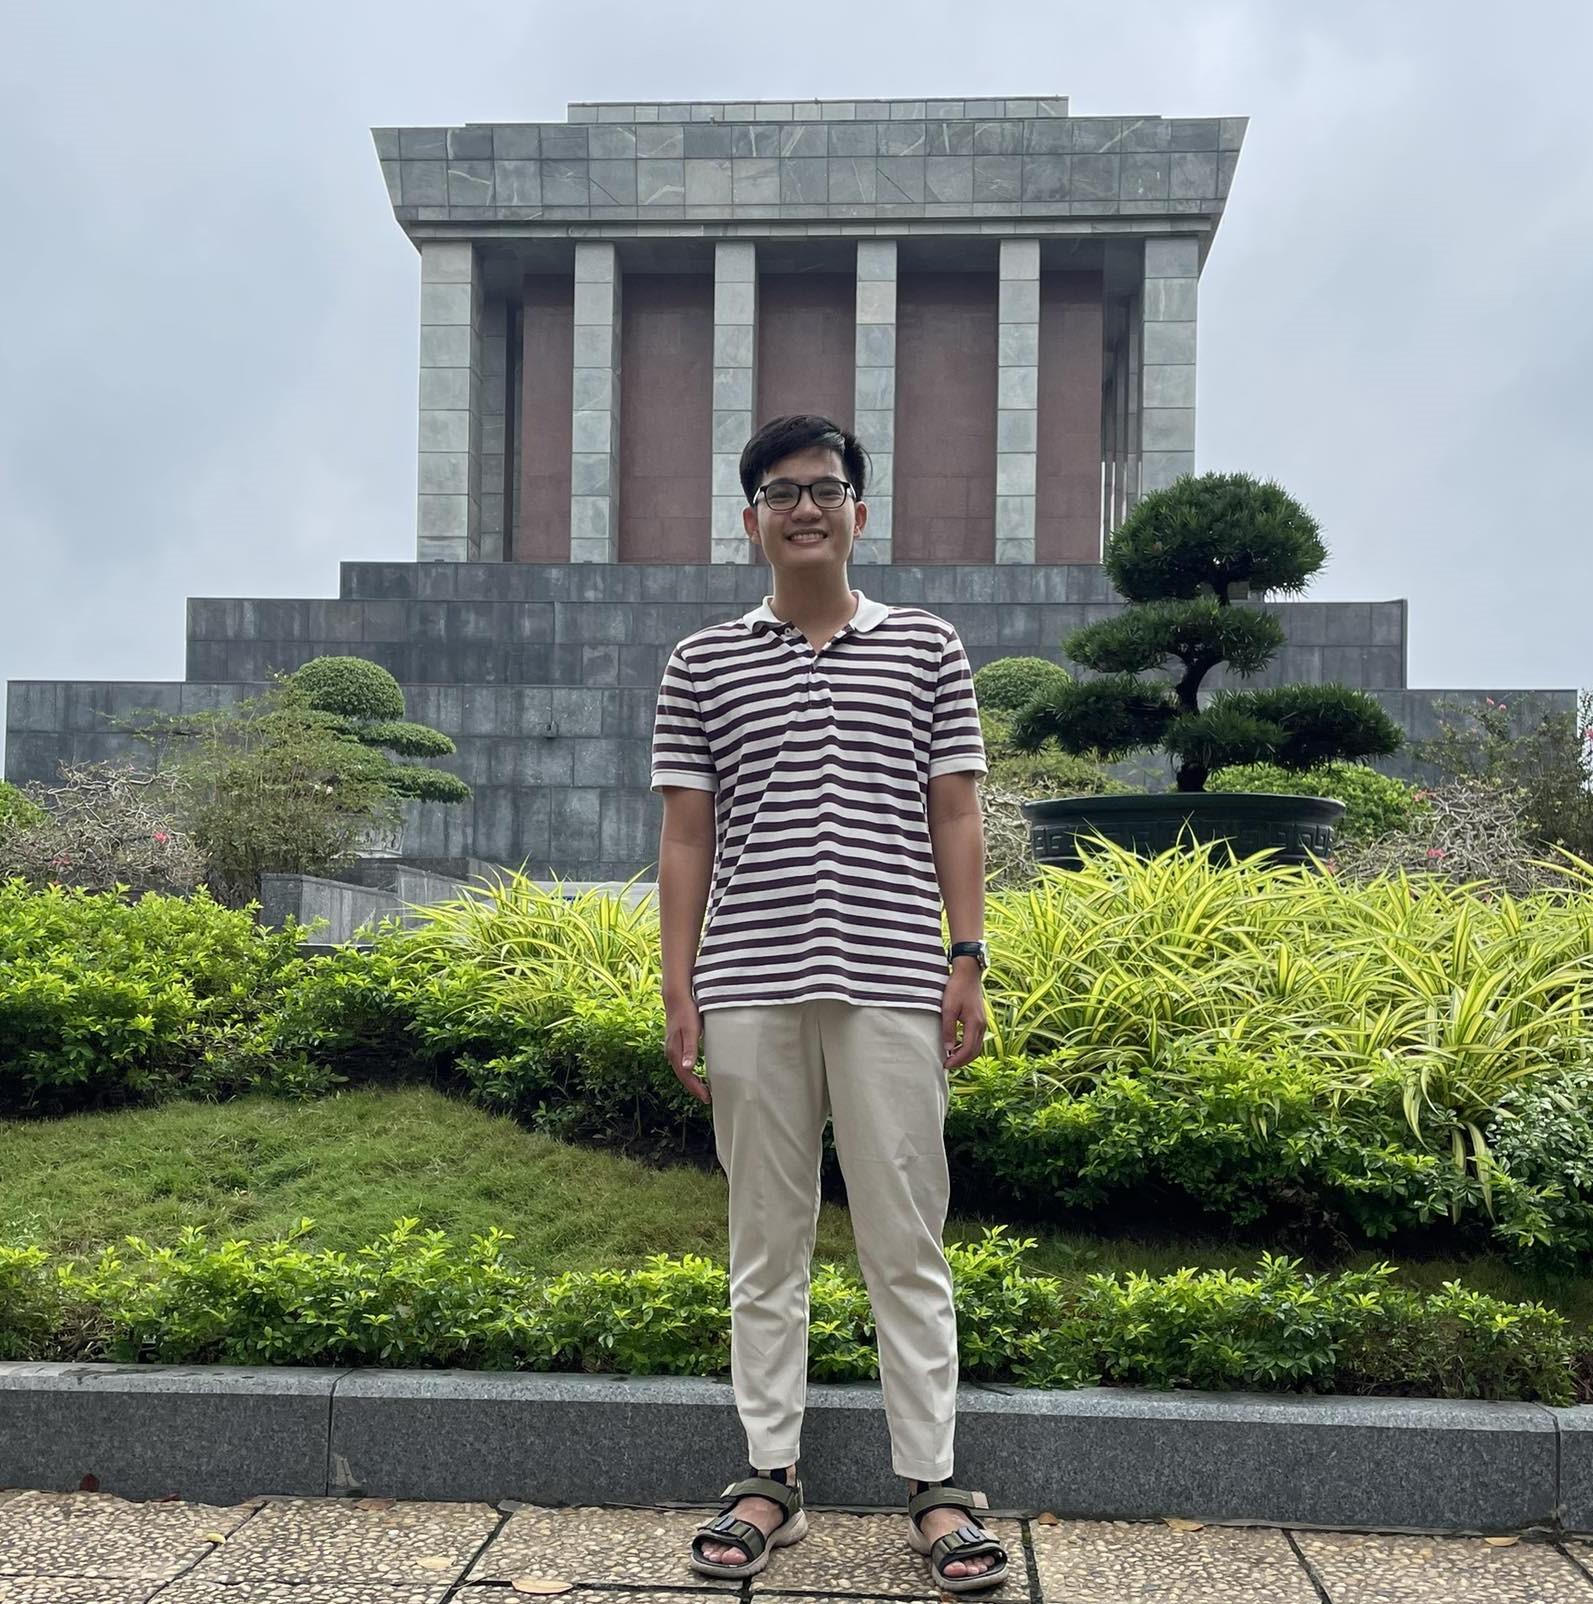
\includegraphics[width=2cm,clip]{logo.jpg}

}\parbox{\dimexpr\linewidth-2.8cm\relax}{
\begin{tabularx}{\linewidth}{L r}
  \textbf{\LARGE \name} & +84-\phone\\
%   {Roll No.:\roll} & \href{mailto:\emaila}{\emaila} \\
  \course &  \href{mailto:\email}{\email}\\
  {Engineer in Automotive industry} &  \href{https://github.com/\github}{Github} $|$ \href{\facebook}{facebook} $|$ \href{https://www.linkedin.com/in/}{linkedin}\\
  {Ho Chi Minh City University of Technology and Education, VietNam} %& \href{\Linkedln}{linkedin}
\end{tabularx}
}



%-----------EDUCATION-----------------
% \section{Education}
%   \resumeSubHeadingListStart
%     \resumeSubheading
%       {Indian Institute of Technology Guwahati}{Guwahati, India}
%       {Bachelor of Technology in Mathematics and Computing ;  GPA: 8.10}{July. 2015 -- July. 2019 (Expected)}
%     \resumeSubheading
%       {Burdwan Model School}{Burdwan, W.B}
%       {Central Board of Secondary Education (Class XII);  Percentage: 96.60}{March. 2015}
%   \resumeSubHeadingListEnd\vspace{-3mm}
\section{Education}
\setlength{\tabcolsep}{5pt} % Default value: 6pt
% \renewcommand{\arraystretch}{1.1} % Default value: 1
\small{\begin{tabularx}
{\dimexpr\textwidth-3mm\relax}{|c|C|c|c|c|}
  \hline
  \textbf{Degree/Certificate } & \textbf{Institute/Board} & \textbf{GPA} & \textbf{Year} & \textbf{Reference No}\\
  \hline
  SPK.BE. Computer Engineering & Ho Chi Minh City University of Technology and Education & 3.22 & 2023 & 2427FD23\\
  \hline
\end{tabularx}}
\vspace{-2mm}

% %-----------EXPERIENCE-----------------
\section{Experience}
  \resumeSubHeadingListStart

    \resumeSubheading
      {XYZ Company Name}{Location}
      {XXXXXXXXXXX \& YYYYYYYYYYYY Intern}{May 2019 - Jul. 2019}
      \resumeItemListStart
    \item {Work Done List 1}
    \item {Work Done List 2}
    % \item {More work done } .....
    \resumeItemListEnd
    
    % \resumeSubheading
    %   {Company A}{Bengaluru, India}
    %   {API Developer \& Machine Learning Intern}{May. 2018 - Jul. 2018}
    %   \resumeItemListStart
    % \item {XXXXXXXXXXXXXXX}
    %     \item {YYYYYYYYYYYYYYYYYY}
    % \resumeItemListEnd
      
  \resumeSubHeadingListEnd
\vspace{-5.5mm}
%-----------PROJECTS-----------------
\section{Projects}
\resumeSubHeadingListStart
    
    \resumeProject
      {Spotify Product Analysis} %Project Name
      {Road to Intern Fair} %Project Name, Location Name
      {Dec. 2023 - Jan. 2024} %Event Dates
      {\href{Link to project}{Drive}} %Website
      \resumeItemListStart
        \item {Project Work Done 1}
        \item {Project Work Done 2}
    \resumeItemListEnd

    \resumeProject
      {React Weather App} %Project Name
      {Road to Intern Fair} %Project Name, Location Name
      {Dec. 2023 - Jan. 2024} %Event Dates
      {\href{Link to github}{Github}} %Website
      \resumeItemListStart
        \item {Project Work Done 1}
        \item {Project Work Done 2}
    \resumeItemListEnd
    
    \resumeProject
      {Project Name 3}
      {Club Name/Professor Name}{Oct. 2023 - Jan. 2024}{\href{Links to Reports}{Reports}}
      \resumeItemListStart
    \item {Work Done 1}
        \item {Work Done 2}
    \resumeItemListEnd
      
  \resumeSubHeadingListEnd
\vspace{-5.5mm}


\section{Skills}
 \resumeHeadingSkillStart
  \resumeSubItem{Programming} % Category
    {Python, C/C++, Java*}
 \resumeSubItem{Category XYZ} % Category
    {Skill A, Skill B, Skill C} % Skills
%  \resumeSubItem{Tools/Frameworks} % Category
%     {Keras, Tensorflow, Pytorch*, ROS, OpenCV}
 \resumeSubItem{Operating Systems}
 {Windows, Linux*} 
  \resumeSubItem{Non Technical}
 {Product Management, Financial Analysis, Consulting} 
\hfill \textit{\footnotesize{* Elementary proficiency}} \hspace{3mm}
 \resumeHeadingSkillEnd


\section{Key courses taken}
\resumeHeadingSkillStart
 \resumeSubItem{Mathematics} % Category
    {Linear Algebra, Basic Calculus, Discrete Maths, Probability \& Random Processes }
 \resumeSubItem{Product Management} % Category
    {Product Matters 3.0} % Skills
\resumeSubItem{Course Category XYZ}
 {Course Name 1, Course Name 2, Course Name 3, Course Name 4}
 \resumeHeadingSkillEnd


\section{Positions of Responsibility}
\vspace{-0.4mm}
\resumeSubHeadingListStart
\resumePOR{Associate Manager} % Position
    {XYZ Club, IIT Guwahati} %Club,Event
    {Apr. 2018 - Apr. 2019} %Tenure Period
    \resumeItemListStart
        \item { Conducted so and so event for this many audience}
    %     % \item { Also responsible for the social media management and various content initiatives of the Club across platforms}
    \resumeItemListEnd
\resumeSubHeadingListEnd
\vspace{-6mm}

\section{Achievements}
\vspace{-0.2mm}
\resumeSubHeadingListStart
\resumePOR{Bronze Medal} % Award
    { XYZ Challenge, ABC Company, FGH City} % Event
    {2018} %Event Year
\resumePOR{JEE Advanced 2021} % Award
    { Secured \textbf{AIR XYZ} among 0.15 million candidates appearing for the test} % Event
    {2021} %Event Year
\resumePOR{JEE Mains 2021} % Award
    { Secured \textbf{AIR XYZ} among 2.2 million candidates appearing for the test} % Event
    {2021} %Event Year

\resumeSubHeadingListEnd
\vspace{-2mm}
% \hspace*{-5mm}\rule{1.035\textwidth}{0.1mm}
\section{Extracurriculars}
\vspace{-0.4mm}
\resumeSubHeadingListStart
\resumePOR{XYZ position} % Position
    { ABC Society} %Club,Event
    {} %Tenure Period
\resumePOR{Student Volunteer} % Position
    { ABC Activity} %Club,Event
    {} %Tenure Period
\resumeSubHeadingListEnd
\vspace{-4mm}

%-------------------------------------------
\end{document}